\documentclass{scrartcl}
\usepackage[top=3cm, bottom=3cm, left=2cm,right=2cm]{geometry} 

\usepackage[english]{babel}
\usepackage[utf8]{inputenc}
\usepackage{mathtools}
\usepackage{esvect}
\usepackage{amssymb}
\usepackage{amsmath}

\usepackage{dcolumn}
\usepackage{booktabs}
\usepackage{tikz}
\usepackage{graphicx}
\usepackage{multicol}
\usepackage{float}
\usepackage{url}

\usepackage[toc, page]{appendix}


\DeclareMathOperator*{\argmin}{argmin} % no space, limits underneath in displays
\DeclareMathOperator*{\argmax}{argmax} % no space, limits underneath in displays

\DeclarePairedDelimiter\abs{\lvert}{\rvert}%
\DeclarePairedDelimiter\norm{\lVert}{\rVert}%

\usepackage{titlesec}
\newcommand{\sectionbreak}{\clearpage}

\usepackage[parfill]{parskip}
\parskip = 4pt

\title{Pattern Analysis - Lecture notes}
\author{Sebastian Rietsch}

\begin{document}
\maketitle
\tableofcontents
\section{Density Estimation}
Let \(p(\vec{x})\) denote a probability density function (pdf) then:
\begin{enumerate}
    \item
        \(p(\vec{x}) \geq 0 \)
    \item
        \(\int\limits_{-\infty}^{+\infty} p(\vec{x}) d\vec{x} = 1 \)
    \item
        \(p(\vec{a} \leq \vec{x} \leq \vec{b}) = \int\limits_{\vec{a}} p(\vec{x}) d\vec{x} \)
\end{enumerate}
The task of density estimation is to obtain from a set of discrete samples/measurements a continuos representation of the underlying pdf.


\subsection{Parametric density estimation}
Make an assumption about the underlying distribution and determine the best fitting distribution parameters from the data. (MLE, Maximum a Positriori Estimation)

\subsection{Non-parametric density estimation: Parzen-Rosenblatt estimator}
The Parzen window estimator interpolates the pdf from the observations in the neighborhood of a position \(\vec{x}\), using an appropriate kernel (or window) function.

\subsubsection*{Short derivation}
Let \(p_R\) denote the probabilty that \(\vec{x}\) lies within region \(R\): \(p_R = \int_R p(\vec{x}) d\vec{x}\).\\
Now assume that \(p(\vec{x})\) is approximately constant in \(R\).
 \[\Rightarrow p_R = p(\vec{x}) \underbrace{\int_R d\vec{x}}_\text{volume of R}\]\\
For example let \(R\) be a d-dimensional hypercube with side length \(h\), then its volume is \(h^d\) and \(p_R \approx p(\vec{x}) \cdot V_R\).

Let \(p_R = \frac{k_R}{N}\), i.e. we determine the probability of making an observation in region \(R\) by counting the samples in \(R\) \((k_R)\) and dividing by the total number of samples. (\(p_R\) is also called the "relative frequency")\\
\[\Rightarrow p(\vec{x}) = \frac{p_R}{V_R} = \frac{k_R}{V_R \cdot N}\]\\
Let us write the Parzen window estimator as a function of a kernel \(k(\vec{x},\vec{x_i})\), then
\[p(\vec{x}) = \frac{1}{Nh^d} \cdot \sum\limits_{i=1}^{N} k(\vec{x}, \vec{x_i})\]
and
\[k(\vec{x}, \vec{x_i}) = \begin{cases} 
    1 & \frac{|\vec{x}_{i,k} - \vec{x}_k|}{h} \leq \frac{1}{2} \\ 0 & \text{otherwise}
\end{cases}\].\\
In any dimension \(k\),  \(\vec{x_i}\) and \(\vec{x}\) are not farther apart than \(0.5\cdot h\).

Equivalently, if we use a (multivatiate) Gaussian kernel:
\[ k(\vec{x}, \vec{x_i}) = \underbrace{\frac{1}{(2\pi)^d |\Sigma|}}_{\text{Volume of Gaussian}} e^{-(\vec{x} - \vec{x_i})^T \Sigma^{-1} (\vec{x} - \vec{x_1})} \;\; \Rightarrow \;\; p(\vec{x}) = \frac{1}{N} \sum\limits_{i=1}^{N} k(\vec{x}, \vec{x_i})\]

\subsubsection*{A note on application}
\begin{itemize}
    \item
        General remark: we obtain a continous pdf, i.e. density estimation converts a list of measurements to a statistical model
    \item
        One specific example: we can sample from a pdf. This means that we have a principled way of generating new/more ... data that behaves/looks similarly to the observations
\end{itemize}

\subsubsection*{Question: How can we (practically) sample from a pdf?}
\begin{enumerate}
    \item
        Convert pdf into cumulative density function (cdf) (\( cdf[i] = cdf[i-1] + pdf[i]\))
    \item
        Draw a uniformly distributed number (\(r\)) between 0 and 1
    \item
        Our sampled value is \(x\), where \(cdf[x] = r\)  
\end{enumerate}

\subsubsection*{How can we determine good window size?}
Let's do a Maximum Likelihood with cross validation. e.g. leave-one-sample-out cross-validation (CV).
\[ p_{h, N-1}^j (\vec{x}) = \frac{1}{N h^d} \sum_{i=1, i \neq j}^{N} k(\vec{x}, \vec{x_i}) \] \\
We estimate the pdf from all samples except \(\vec{x_j}\). \(\vec{x_j}\) will be used to evaluate the quality of the pdf using window size h.
\begin{align*}
\hat{h} &= \argmax_h \mathcal{L}(h) = \argmax_h \prod_{j=1}^{N} p_{h, N-1}^j (\vec{x_j})\\
&= \argmax_h \sum\limits_{j=1}^{N} log \; p_{h, N-1}^j (\vec{x_j})
\end{align*}
The position of the maximum (when using log-likelihood) does not change, because the logarithm is a strictily monotonic function.

\section{Mean Shift Algorithm (Comaniciu, Meer)}
\textbf{Purpose}: Find maxima in a pdf without actually performing a full density estimation (e.g. for Clustering (maximum is cluster center), segmentation, ...)

Assume that we have a full density estimator. Then 
\[p(\vec{x}) = \frac{1}{N} \sum\limits_{i=1}^N k_h (\vec{x}, \vec{x_i}) \].\\
\textbf{Idea}: Maxima can be found where the gradient of the pdf is zero.\\
\textbf{Problems}:
\begin{itemize}
    \item
        It may be the case, that a zero gradient is just between two finer maxima
    \item
        The kernel size indirectly controls the number of identified maxima
\end{itemize}

\textbf{Applications:}
\begin{itemize}
    \item
        Clustering: Find local maxima, create one cluster per maxima  and assign every vector to the maxima it "walks up to" (gradient points in direction of maxima)
    \item
        Image smoothing: define features as \(x_i = (x, y, L, u, v)^T\), assign pixels forming a cluster to the mean Luv-value
\end{itemize}


\section{Mean Shift Algorithm (continued)}
Let 
\[p(x) = \frac{1}{N} \sum_{i=1}^N K_{h}(x_i, x)\]
denote the multivariate kernel density estimate.

A local maximum of the PDF can be assumed where the gradient \(\bigtriangledown p(x) = 0\) ("the gradient vanished", local minimum not possible because we perform a grandient asscend).

\[\bigtriangledown p(x) = \bigtriangledown(\frac{1}{N} \sum_{i=1}^N K_h (x_i,x)) = \frac{1}{N} \sum_{i=1}^N \bigtriangledown K_h(x_i, x)\]

Let us assume that \(K_h\) is a radially symmetric kernel, i.e. 
\[K_h(x_i, x) = c \cdot k_h(\norm{x_i -x}^2)\]
where \(c\) is a constant that adjusts this quantity towards \(d\) dimensions.

\[\frac{\partial k_h(s)}{\partial s} = k_h'(s)\]
\[\frac{\partial k_h(s)}{\partial x} = \frac{\partial (x_i -x)^T(x_i -x)}{\partial x} = -2 (x_i - x)\]

\[\Rightarrow \bigtriangledown p(x) = \frac{1}{N} \cdot \sum_{i=0}^N c_d \cdot k_h'(\norm{x_i - x}^2) \cdot (-2 (x_i - x)) = \vec{0}\]

(drop \(\frac{1}{N}, c_d)\), multiply)

\[\Leftrightarrow \sum_{i=1}^N k_h'(\norm{x_i -x}^2) \cdot x_i - \sum_{i=1}^N k_h'(\norm{x_i -x}) \cdot x = \vec{0}\]

Mean shift vector:
\[\frac{\sum_{i=1}^N k_h'(\norm{x_i -x}^2) \cdot x_i}{\sum_{i=1}^N k_h'(\norm{x_i-x}^2)} - x = \vec{0}\]

Mean Shift Algorithm:
\begin{enumerate}
    \item
        Compute mean shift vector  
    \item
        Update \(x\):         
        \begin{align*}
            x^{(t+1)} &= x^{(t)} + m(x^{(t)})\\
            &= x^{(t)} + \frac{\sum_{i=1}^N k_h'(\norm{x_i^{(t)} -x^{(t)}}^2) \cdot x_i^{(t)}}{\sum_{i=1}^N k_h'(\norm{x_i^{(t)}-x^{(t)}}^2)} - x^{(t)} 
        \end{align*}
\end{enumerate}

Why is it called "Mean Shift"? Because if we plug in for \(k_h\) the Epanechnikov kernel,  the whole computation breaks down to computing for the update the mean of the samples in a circular or (hyperspherical, resp.) neighborhood around \(x^{(t)}\).

Epanechnikov kernel: \(k_{E} (x) = 
\begin{cases} 
    c \cdot (1-x^Tx) & x^Tx \leq 1\\
    0 & otherwise
\end{cases}\) 

\textbf{Example applications:}
\begin{enumerate}
    \item
        (Color) quantization
    \item
        Segmentation: similar in result to a superpixel segmentation: operate locally in the image \(\Rightarrow\) incorporate the position of each pixel. Thus, the feature vector becomes 5-dimensional, consisting of \((x, y, r, g, b)\). Properly scale each feature dimension, such that distances are comparable between them.
\end{enumerate}

\textbf{Remarks} on the found maxima:
\begin{enumerate}
    \item
        Different trajectories typically converge only to \underline{almost} the same peak, thus we will have to postprocess the peaks and (somewhat) reduce them
    \item
        We do not have a guarantee to sit on top of a maximum when reaching a 0-gradient. This is due to the finite window size and the discrete representation of our density
    \item
        If the amount of data is larger, then it may become extremely costly to iteratively evaluate the "neighborhood finder." In that case, you have to help yourself either with a smart data structure or LSH (Locality-Sensitive Hashing)
\end{enumerate}

Note: RGB color space is not perceptually uniform. This means the same Euclidean distance between two points looks very different for different point pairs in RGB space. Standard way out: Lab or Luv color space.

\section{Clustering}
Summary: Elements of Statiscial Learning, Section 14
\subsection{Cluster Analysis}
Grouping or segmenting a collection of objects into subsets or "clusters", such that those within each cluster are more closely related to one another than objects assigned to different clusters. Sometimes the goal also is to arrange the clusters into a natural hirarchy.

All clustering methods attempt to group the objects based on the definition of similarity supplied to it \(\rightarrow\) choice of distance or dissimilarity measure between two objects.

\subsubsection{Proximity Matrices}
Sometimes the data is represented directly in terms of the proximity (alikeness or affinity) between pairs of objects. These can either be \textit{similarities} or \textit{dissimilarities}. This type of data can be represented by an \(N \times N\) matrix \(D\), where \(N\) is the number of objects, and each element \(d_{ii'}\) records the proximity between the \(i\)th and \(i'\)th objects.

Most algorithms presume a symmetric matrix of dissimilarities with nonnegative entries and zero diagonal elements. If the original data were collected as similiarities, a suitable monotone-decreasing function can be used to convert them to dissimilarities.

\subsubsection{Dissimilarities Based on Attributes}
Most often we have measurements \(x_{ij}\) for \(i = 1, \dots, N\), on variables \(j=1,\dots, p\) (also called \textit{attributes}. We first have to construct pairwise dissimilarities between the observations. In the common case, we define a dissimilarity \(d_j(x_{ij}, x_{i'j})\) (e.g. squared distance \((x_{ij} - x_{i'j})^2\), even though not appropriate for nonquantitive/categorial attributes) between values of the \(j\)th attribute, and then define
\[D(x_i, x_i') = \sum_{j=1}^p d_j(x_{ij}, x_{i'j})\]

\begin{itemize}
    \item
        Ordinal variables: Convert to numbers on a scale 
    \item
        Categorial(nominal) variables: Dissimialrity has to be described explicitly
\end{itemize}

\subsubsection{Object Dissimilarity}
For comparing objects, often a weighted sum of distances is computed:
\[D(x_i, x_i') = \sum_{j=1}^p w_j d_j(x_{ij}, x_{i'j}); \sum_{j=1}^p w_j = 1\]

Note that giving every variable the same weight \(w_j\) doesn't necessarily give all attributes equal influence. The relative influence of the \(j\)th variable is given by \(w_j \cdot \bar{d_j}\), where \(\bar{d_j} = \frac{1}{N^2} \sum_{i=1}^{N}\sum_{j=1}^{N}d_j(x_{ij}, x_{i'j})\) is the average dissimilarity on the \(j\)th attribute. To achieve this the weights have to be set to \(w_j = \frac{1}{\hat{d_j}}\), which doesn't always make sense.

Specifying an appropriate dissimilarity measure is far more important in obtaining success with clustering than choice of clustering algorithm.

\subsubsection{Clustering Algorithm}
Three types of clustering algorithms:
\begin{itemize}
    \item
        \textbf{Combinatorial:} work directly on the observed data with no direct reference to an unterlying probability model.
    \item
        \textbf{Mixture modeling:} suposes that the data is a sample from some population describe by an probability density function. This density function is characterized by a parameterized model taken to be a mixture of component density functions; each component density describes one of the clusters.
    \item
        \textbf{Mode seeking("bump hunting"):} take a nonparamteric perspective, attempting to directly estimate distinct modes of the pdf. Observations "closest"to each respective mode then define the individual clusters.
\end{itemize}
\subsubsection{Combinatorial Algorithms}
Each observation is uniquely labeled by an integer \(i \in \{1, \dots N\}\). A prespecified number of clusters \(K<N\) is postulated, and each one is labeled by an integer \(k \in \{1, \dots, K\}\). Each observation is assigned to one and only one cluster by an "encoder" \(C(i) = k\), that assigned the \(i\)th observation to the \(k\)th cluster. One seeks the particular encoder \(C^*(i)\) that achieves the required goal, based on the dissimilarities between every pair of observations.

One approach is to directly specify a mathematical loss function and attempt to minimize it through some combinatorial optimization algorithm. Since the goal is to assign close points to the same cluster, a natural loss function would be 
\[W(C) = \frac{1}{2} \sum_{k=1}^K \sum_{C(i)=k}\sum_{C(i')=k} d(x_i, x_{i'})\]
which is also called the \textit{within-cluster scatter}. One can equivalently maximize the \textit{between-cluster scatter}
\[B(C) = \frac{1}{2} \sum_{k=1}^K \sum_{C(i)=k}\sum_{C(i') \neq k} d(x_i, x_{i'})\]

One simple way to solve this is to minimizes \(W\) or maximized \(B\) over all possible assignments of the \(N\) data points to \(K\) clusters. Unfortunally, such optimization by complete enumeration is feasible only for very small data sets.

For this reason, practical clustering algorithms are able to maximize only a very small fraction of all possible encoders \(C\). The goal is to identify a small subset that is likely to contain the optimal one, or at least a good suboptimal partition. Such feasible stratgies are based on iterative greedy descent (initial partition is specified, at each step cluster assignments are changed such that value of criteroen is improved, stop when no more improvement possible).

\subsubsection{K-means}
Squared Euclidean distance:
\[d(x_i, x_{i'}) = \sum_{j=1}^p (x_{ij} - x_{i'j})^2 = \norm{x_i - x_{i'}}^2\]

The within-point scatter can be written as
\[W(C) = \sum_{k=1}^K N_k \sum_{C(i) = k} \norm{x_i - \bar{x_k}}^2\]
where \(\hat{x_k}\) is the mean vector associated with the \(k\)th cluster, and \(N_k\) is the number of observations assigned to a cluster. Thus, the critereon is minimized by assigning the \(N\) observations to the \(K\) clusters in such a way that within each cluster the average dissimilarity of the observations from the cluster mean, as defined by the points in that cluster, is minimized.

\bigbreak

\textbf{Algorithm:}
\begin{enumerate}
    \item
        For a given cluster assignment \(C\), compute each clusters mean
    \item
        Assign each observation to the closest cluster mean
    \item
        Iterate 1 and 2 until the assignments do not change
\end{enumerate}

Each iteration reduces the value of the critereon, so that convergence is assured, but the solution may be suboptimal. In addition, on should start the algorithm with many different random choices for the starting means, and choose the solution having smallest value of the objective function.

\subsubsection{Gaussian Mixtures as Soft \(K\)-means Clustering}
The \(K\)-means clustering procedure is closely related to the EM algorithm for estimating a certain Gaussian mixture model. Suppose we specify \(K\) mixture components, each with a Gaussian density having a scalar covariance matrix \(\sigma^2 I\). Then the relative density under each mixture component is a monotone function of the Euclidean distance between the data point and the mixture center. Hence in this setup EM is a "soft" version of \(K\)-means clustering, making probabilistic assignments of points to cluster centers. As the variance \(\sigma^2 \rightarrow 0\), these probabilities become 0 and 1, and the two methods coincide (responsibility of mixture component \(i: \frac{g_i(x)}{\sum_m g_m(x)}\)).

\subsubsection{Vector quantization}
The \(K\)-means clustering algorithm represents a key tool in the apparently unrelated area of image and signal compression, particular in \textit{vector quantization} or \textit{VQ}(Gersho and Gray, 1992). 

\textbf{Algorithm}:
\begin{enumerate}
    \item
        Convert to grayscale
    \item
        Break image into small blocks, e.g. \(2 \times 2\) blocks of pixels
    \item
        Each block is regarded as a vector in \(\mathcal{R}^4\)
    \item
        Apply \(K\)-means
    \item
        Each of the blocks is approximated by its closest cluster centroid, known as codeword. The clustering process is called the \textit{encoding} step, and the collection of centroids is called the \textit{codebook}.
\end{enumerate}

\subsubsection{\(K\)-medioids}
 \(K-\)means stuggels with outliers, because using \textit{squared} Euclidean distance places the highest influence on the larger distances.

 Instead of taking means as cluster center, one can identify the sample inside each cluster, which is nearest to all other samples inside it. One then assigns this sample to be the new cluster center.

 The downside is that \(K\)-medioids is far more computationally intensive.

 \subsubsection{Practical Issues}
 In order to use \(K\)-means or -medioids one must select the number of clusters \(K^*\) as initialization. A choice for the number of clusters \(K\) depends on the goal. For data segmentation \(K\) is usually defined a part of the problem.

 Data-based methods for estimating \(K^*\) typically examine the within cluster dissimilarity \(W_k\) as a function of the number of clusters \(K\). Seperate solutions are obtained for \(K \in \{1,2,\dots,K_{max}\}\). The corresponding values generally decrease with increasing \(K\). 

\bigbreak
 
\textbf{Intuition:}
\begin{itemize}
    \item
        \(K < K^*\) will partition actual groups into subsets. The solution criterion value will tend to decrease substantially with each successive increase in the number of specified clusters, \(W_{K+1} \ll W_K\), as the natural groups are successively assigned to seperate clusters.
    \item
        \(K > K^*\) will fuse natural groups into one. This will tend to provide a smaller decrease in the criterion as \(K\) is further increased.
\end{itemize}
\(\Rightarrow\) Splitting a natural group, within which the observations are quite close to each other, reduces the criterion less than partitioning the union of two well-separated groups into their proper constituents.

To the extent this scenario is realized, there will be a sharp decrease in successive differences in critereon value, \(W_K - W_{K+1}\), at \(K=K^*\). An estimate for \(K^*\) is then obtained by identifying a "kink" in the plot of \(W_K\) as a function of \(K\). As with outher aspects of clustering procedures, this approach is somewhat heuristic.

Recently proposed \textit{Gap statistic} (Tibshirani et al., 2001b): 
\begin{itemize}
    \item
        Compare the curve \(log W_K\) to the curve obtained from data uniformily distributed over a rectangle containing the data.
    \item
        Optimal \(K\) is where the gap between the two curves is largest
\end{itemize}
                
\subsubsection{Hirarchical Clustering}
Hirarchical clustering methods do not require specifications like for \(K\)-means. Instead, the require the user to specify a measure of dissimilarity between (disjoint) \textit{groups} of observations, based on the pairwise dissimilarities among the observartions in the two groups.

At the lowest level, each cluster contains a single observation. At the highest level there is only one cluster containing all of the data.

Two basic paradigms: \textit{aglomerative} (bottom-up, every step up there is one less cluster) and \textit{devisive} (top-down, every step down there is one new cluster). There are \(N-1\) levels in the hirarchy.

\textbf{Agglomerative Clustering}

Let \(G, H\) represent two groups. The dissimilarity \(d(G,H)\) is computed from the set of pairwise observation dissimilarities \(d_{ii'}\).\textit{Single linkage} (SL) agglomerative clustering takes the intergroup dissimilarity to be that of the closest (least dissimilar) pair. This is also often called the \textit{nearest-neighbor} technique. \textit{Complete linkage} (CL) agglomerative clustering (\textit{furthest-neighbor} technique) takes the intergroup dissimilarity to be that of the furthest pair. \textit{Group average} (GA) clutering uses the average dissimilarity between the groups (trade-off between compactness/diameter of clusters).

\section{Dirichlet Process}
We have several options for clustering the data. \(k-\)means variants are straight forward, easy to understand, but if the proper number of clusters is part of the unknowns, it may be a suboptimal choice. One alternative is mean shift clustering: here, the number of clusters is determined implicitly by the kernel type and size, and the type of bump post processing (non-maximum supression).

Today, we will look into a \textbf{Dirichlet Process} to model infinite Gaussian mixtures.

\bigbreak

Short reminder: Gaussian mixture models.
\begin{enumerate}
    \item
        What is a GMM? \(\Rightarrow \sum_{i=1}^k \beta_i \mathcal{N}(\mu_i, \Sigma_i)\)
    \item
        What parameters? \(\Rightarrow \beta_i, \mu_i, \Sigma_i\) 
    \item
        How do I determine these parameters? \(\Rightarrow EM-Algorithm\)

        Start with random initialization, expectation (how much does each component contribute to each point), maximization (update component parameters), repeat until convergence

        From a more abstract perspective, EM performs two tasks simultaneously: segmentation/clustering assignment, and model parameters estimation/fitting
\end{enumerate}

\bigbreak

Idea for infinite mixture models: Instead of fitting a specific distribution to the data (the GMM), we define a meta-distribution from which the actual distribution is drawn. The infinite mixture model can be used for clustering.

Specifically, we can draw a GMM from a Dirichlet Process. However, this is a top-down persepectiv, i.e., if we randomly draw a GMM, we will certainly not draw one the nicely fits to our data. From a bottom-up perspective, we need a fitting algorithm that works with the available data points and finds a GMM in such a way that it could also have been drawn from a distribution of distribtions (the Dirichlet Proess).

To illustrate the model behind the fitting algorithm, we usually talk about the \textbf{Chinese Restaurante Process}.

\begin{itemize}
    \item
        There are tables in a restaurant (our mixture components)
    \item
        Whenever a new customer comes in (a sample), it chooses the table it most relates to
    \item
        When the customer is unsatisfied with current offering, he can open up a new table
\end{itemize}

Extension to a "normal" GMM:
\begin{enumerate}
    \item
        If a customer prefers to sit on a new table, this is possible: we can add arbitrarily many tables (this will vary the \(k\) in our mixture model)
    \item
        "Rich get richer":
        The more people sit on a table, the more attractive it is to new customers ("this must be really tasty")
\end{enumerate}

%If we adopt the chinese restaurante process, we are essentially following the rules for sampling from a Dirichlet process.
The Chinese Restaurant Process (CRP) provides a constructive way of sampling from a Dirichlet Process.

Here is a straight forward clustering algorithm based on the CRP:

\begin{enumerate}
    \item
        Init: assign each sample to a cluster (e.g. randomly, or do \(k-\)means)
    \item
        Randomly select a sample \(x_i\) from the data
    \item
        Compute a affinity of \(x_i\) to each table: \(t_i = \frac{N_i}{N+\alpha} \mathcal{N}(x_i, \mu_i, \Sigma_i)\) (Gaussian distance of \(x_i\) to \(\mathcal(\mu_i, \Sigma_i)\)), where \(N_i\) is the number of customers on the table (number of samples assigned to \(\mathcal{N}(\mu_i, \Sigma_i)\) and \(N\) is the total number of samples, \(\alpha\) is an "expansion parameter"
    \item
        Compute affinity to a new table \(t_0 = \frac{\alpha}{N + \alpha} \cdot \mathcal{N}(x_i, \mu_0, \Sigma_0)\)
    \item
        Collect all affinities \(t_0, \dots, t_T\) in a list, normalize sum to one
    \item
        Sample from that list a table assignment (all affinities are interpreted as a PDF from which we sample)
    \item
        Recompute \(\mu_i, \Sigma_i\) for the assigned table
    \item
        Goto 2, stop after certain number of iterations
\end{enumerate}

This type of algorithm is called \textbf{Gibbs sampling} (take one out, modify, put it back). This is a probabilistic algorithm (we sample from the list of affinities).

\section{Dirichlet Process (continued)}
Criteria for the affinity of a sample \(x\) to a cluster \(\vartheta_i\):
\begin{itemize}
    \item
        Proximity: \(\mathcal{N}(x, \mu_i, \Sigma_i)\)
    \item
        Number of samples already assigned to that cluster: \(\frac{N_i}{N+\alpha}\), where \(\alpha\) is the expansion parameter (corresponds to \(\beta\) in Gaussian Mixture, \(G = \sum_{i=0}^k \beta_i \mathcal{N}(\mu_i, \Sigma_i)\)
\end{itemize}
Back to our top-down view: using the \textit{CRP}, we are effectively drawing a fully parameterized GMM using a Dirichlet Process. Implicitly, the mixture weights \(\beta_i\) match a Beta(\(\alpha\)) distribution and the Normal-distributions are drawn from hyper-distribution i.e. \(\vartheta_i \sim H(\lambda)\).

\bigbreak

Illustration of a Beta-distribution: Stick breaking process:

\begin{enumerate}
    \item
        Stick of length 1 
    \item
        We draw a random number between 0 and 1
    \item
        We break this length off from the stick
    \item
        Repeat 2,3 infinitly, while scaling the random number down to new sick length
    \item
        The length of the stick parts are our cluster weights
\end{enumerate}

We draw from a \(Beta (1,\alpha) = \frac{\Gamma(a) \cdot \Gamma(\alpha)}{\Gamma(1+\alpha)}\) distribution, where \(\Gamma(x) = \int_0^{\infty} u^{x-1}e^{-u}du \) is a Gamma-distribution.

We are expressing the probability distribution for flipping a coin, but the coin doesn't need to be fair (if the two parameters are far apart, it's a unfair coin. If they are close, it's more fair).

Qualitatively, this is what Beta-distribution looks like:
\begin{center}
    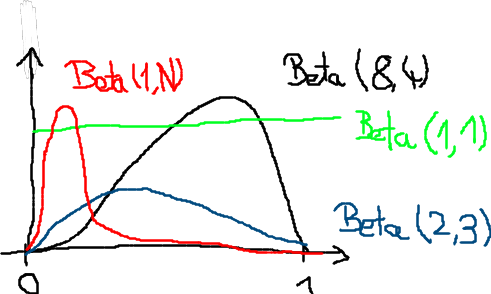
\includegraphics[scale=0.7]{img/betadist.png}
\end{center}
The expansion parameter \(\alpha\) is a prior, that influences the number of clusters that will be created. 

\textbf{Observation 1:} The larger the expansion parameter \(\alpha\) is, the more likeli it is to draw a number that is close to zero from \(Beta(1,\alpha)\).

\textbf{Observation 2:} The number that has been drawn from \(Beta(1,\alpha)\) is used in the stick breaking process to determine the weight of the \(i\)-th mixture component \(\beta_i\).

Stick breaking process:
\begin{itemize}
    \item
        \(b_i \sim Beta(1, \alpha)\)
    \item
        \(\beta_i = b_i \cdot \prod_{l=1}^{i-1} (1-b_l) = b_i \cdot (1-\sum_{l=1}^{k-1} \beta_l\) (remaining stick length)
\end{itemize}

\section{Manifold Learning}
\subsection{Curse of Dimensionality}
"Human intuition breaks down in high dimensional spaces." (Bellman, 1961)

Let us illustrate this: Consider \(d\)-dimensional feature vectors \(x_1, x_2, \dots, x_n \in \mathcal{R}^d\) where \(0 \leq x_{i,k} \leq 1\) uniformly distributed in a \(d\)-dimensioanl hypercube of volume \(1\). Let's say we would like to cover enough volume of that cube to collect \(1\%\) of the data. Let's say we also use a cube for this task. What is the required edge length of the cube to obtain that \(1\%\) of space?
\begin{itemize}
    \item
        For example, for a 10-dimensional hypercube: 
        \[V = s^d \Rightarrow s = V^{\frac{1}{d}} = 0.01^{\frac{1}{10}} = 0.63\] 
\end{itemize}
Another perspective: We have to draw a \(10\)-dimensional vector, where no value is allowed to exceed \(0.63\) (has probabiliy of \(1\%\)).

Another way of thinking about this is thtat in a high dimensional space, virtually every feature point is located at the boundary of the space, because in at least one dimension we draw a very low or very high value. This leads to the effect that common distance measures loose their effectivity.

This can be seen by looking at the \underline{median} distance of the nearest neighbor to the origin, given \(N\) samples in \(d\) dimensions:
\[medianDist(d, N) = (1 - \frac{1}{2}^{\frac{1}{N}})^{\frac{1}{d}}\]
\[\Rightarrow N=5000, d=10: medianDist(10, 5000) \approx 0.52\]

This shows that distance measures start losing their effectiveness to measure dissimilarity in high dimensional spaces. Because of this, we need methods for reducing the dimensionality of our data, witout breaking its structure to hard.

\bigbreak

"Notorious" example for high dimensional data: \textit{hyperspectral remote sensing image classification}

Satellite image: perfom e.g. aggricultural monitoring: classify type of vegetation via hyperspectral vector (dozens of color channels).

In such classification pipelines, dimensionality reduction is often times one integral component.

\subsection{(k)PCA}

Our known approach to dimensionality reduction: \textbf{PCA} (principle component analysis): We search for an orthogonal basis that is aligned with the "maximum spread" (w.r.t to the covariance of the data). It is a global and unsupervised methode, operating on all datapoints (no labels, finds on globally optimal solution).

PCA is a linear method, which is problematic in certain cases \(\Rightarrow\) Kernel PCA: perform a non-linear mapping of the data, then perfom stadard (linear) PCA on the result. For radial data (inner and outer circle of two classes) we can for example perform a radial transform (space consisting of radius and angle). With the kernel trick, the non-linear mapping and PCA can be merged into one step.

\textit{Objective fuction:} \[J = \sum_{i,j=1}^N(\Phi(x_i) - \Phi(x_j))^T (\Phi(x_i) - \Phi(x_j)) - \lambda(\Phi^T \Phi - 1)\]
where nonlinear mapping is part of the \(\Phi\).

The \textbf{kPCA} idea had some successfull offsprings:
\begin{enumerate}
    \item
        perform some preprocessing/mapping that operates \underline{non-linearly}
    \item
        the dimensionality reduction itself is an operation that operates linearly (linear algebra)
\end{enumerate}

PCA operates on explicitly given feature vectors \(x_i\). What if we only have access to differences between feature vectors, such as the Euclidean distance \(\norm{x_i - x_j}_2^2\)?

\(\Rightarrow\) This is a closely related problem, PCA on distances is called \textbf{MDS}.

\subsection{Multidimensional Scaling (MDS)}
\textit{Task:} Reconstruct a set of points (potentially in a lower dimension) from their differences. MDS computes the "best" (in a least square sense) coordinates up to rotation, translation and mirroring (axis reversal).

\textit{Mathmatical problem formulation:}
\begin{itemize}
    \item
        Let \(S = \{x_1, \dots, x_N\}, x_i \in \mathbb{R}^d\). 
    \item
        Let \(X\) denote a matrix consisting of all samples, \(X=[x_1, \dots, x_N] \in \mathbb{R}^{d \times N}\).
    \item
        Let \(D^2 = [d_{ij}^2]_{i, j \in \{1, \dots, N\}}\), where \(d_{ij}^2 = (x_i - x_j)^T (x_i - x_j)\). 
    \item
        Goal: Given \(D^2\), compute \(X\).
    \item
        We assume that \(x_1, \dots, x_N\) have zero mean i.e. \(\sum_{i=1}^N x_i = 0\)
\end{itemize}

Let us consider the distance matrix in terms of \(x\):
\[d_{ij}^2 = (x_i - x_j)^T(x_i - x_j)=x_i^T x_i + x_j^T x_j - 2 x_i x_j\]

In matrix notation,
\[D^2 = diag(X^T X) \cdot \vec{1}^T + \vec{1} \cdot diag(X^T X)^T - 2X^TX\]
where \(diag(A)\) denotes a vector diagonal entries of \(A\), i.e. \(diag(A) = (a_{11}, a_{22}, \dots, a_{NN})^2\), and \(\vec{1}\) denotes a vector of ones, i.e. \(\vec{1} = (1,1,\dots,1)^T \in \mathbb{R}^d\).

Multiply \(D^2\) from left and right with a centering matrix \(C = (I - \frac{1}{N} \vec{1} \ \vec{1}^T)\), and weight the result by \(-\frac{1}{2}\):
\begin{align*}
    -\frac{1}{2} C D^2 C &= -\frac{1}{2} (I- \frac{1}{N} \vec{1} \ \vec{1}^T) (diag(X^T X) \cdot \vec{1}^T + \vec{1} \cdot diag(X^T X)^T - 2X^TX)(I- \frac{1}{N} \vec{1} \ \vec{1}^T)\\
    &= \dots (\text{see lecture, too lazy}) \\
    &= X^T X
\end{align*}

This is a matrix factorization problem. If you you compute \(SVD(X^T X) \Rightarrow U \Sigma V \Rightarrow X = \Sigma^{\frac{1}{2}} V\).

MDS is essentially the same thing as PCA, but it operates on distances. We can reduce the dimensionality of our data by:
\begin{itemize}
    \item
        Determining the \(m\) largest eigennvalues and their corresponding eigenvectors
    \item
        Dropping the remaining eigenvalue and eigennvectors inside the multiplication
\end{itemize}

\subsection{ISOMAP algorithm}
A non-linearity "patch" for MDS. 

Idea: nearby points have their "usual" Euclidean distance. If a pair of points is not within a local neighborhood, the distance between these points is a graph distance (shortest path). We have an all pairs shortest path problem, which can be solved with certain algorithms (Dijstra, \(A^*\), BFS, DFS, ...). Then, run MDS on the resulting distance matrix. 

This procedure is useful if you want to reduce the dimensionality of "swirly" datasets for example.

ISOMAP operates on geodesic distances (like a distance on earths surface). This means that 

\subsection{Locally Linear Embedding}
\textit{Idea:} Treat the local neighborhood of a point \(x\) as linear. This makes the mapping an overall non-linear mapping consisting of small linear patches.

We can linearily interpolate a point \(x_i\) from its neighbors,
\[x_i = \sum_{x_j \in N(x_i), j \neq i} w_{ij} x_j, \text{ subject to } \sum_j w_{ij} = 1\]
and search points \(x'\) in a lower dimensional space, such that
\[x_i' = \sum_{j \in N(x_i')} w_{ij} x_j'.\]

\textbf{Algorithm:}
\begin{enumerate}
    \item
        Define the neighborhood (\(k\)-nearest neighbors, distance thresholding) 
    \item
        Solve for \(w_{ij}\) in the high dimensional space 
        \[min \sum_{i}\norm{x_i - \sum_{j\in N(x_i)} w_{ij} x_j}_2^2 \text{ subject to } \sum_{j \in N(x_i)} w_{ij} = 1\]%, \ \ \  \forall i \in \{1, \dots. N\}\]
    \item
        Solve for \(x_i' \in \mathbb{R}^{d'} (d' \ll d)\):
        \[\sum_i \norm{x_i' - \sum_{j \in N(x_i)} w_{ij} x_j'}_2^2, \text{ subject to } \frac{1}{N} \cdot \sum_i x_i' \cdot x_i'^T = I, \sum_i x_i' = \vec{0}\]
        The first constraint says that the covariance is the identity.
\end{enumerate}
Nearer point in the original space will result in higher weights.

\textit{Caveats:} 
\begin{enumerate}
    \item
        The idea of LLE is really nice, but the original formulation is sometimes a bit unstable if applied on real data. Therefore there exists a number of variants to LLE in the literature that aims to make it more robust.
    \item
        We will now deviate from the original formulation, and modify the constraint in step 2 to \(\sum_{j in N(x_i)} w_{ij}^2 =1\), to obtain a closed solution.
\end{enumerate}

\bigbreak

\textit{Modified step 2} (weight computation): Note tha the objective function is \underline{invariant} to translation: 
\begin{align*}
    \sum_{i=1}^N \norm{x_i - \sum_j w_{ij} x_j}_2^2 &= \sum_{i=1}^N \norm{(x_i - \vec{t}) - \sum_j w_{ij} (x_j - \vec{t})}_2^2\\
    \Rightarrow \text{set } x_i = \vec{t} & \Rightarrow 
\sum_{i=1}^N \norm{\sum_j w_{ij} (x_j - x_i)}_2^2\\
    = \norm{M_i\vec{w_i}}_2^2, \text{ where } 
    \vec{w_i} &= \left( \begin{array}{c} w_{i1} \\ w_{i2} \\ \dots \\ w_{iN} \end{array} \right)
   , M_i = \left(\begin{array}{cccc} x_1 - x_i & x_2 - x_i& \dots& x_N - x_i \end{array}\right)\\
\end{align*}
Note: differences \(x_j - x_i = 0\) for \(x_j\) outside the neighborhood of \(x_i\)
\[\Rightarrow minimize (M_i w_i)^T (M_i w_i) + \lambda(1-w_i^T w_i), w.r.t \ w_i\]
where the latter is the constraint that the squared weights should sum up to one. We see why we have to take the squaered weights critereon: if we would compute the derivative of \(\lambda(1-w_i)\), the constraint would vanish to \(0\). We would have to use linear programming or something.

Compute 
\[\frac{\partial}{\partial w_i} (w_i^T (M_i^T M_i) w_i + \lambda(1-w_i^T w_i)=  2 \cdot M_i^T M_i w_i - 2 \lambda  \cdot w_i = 0\]
\[\Rightarrow M_i^T M_i w_i = \lambda w_i\]

This is an eigenvector eigenvalue problem and can solve this easily.


\section{Random Forests}
\textit{What is a random forest?} An ensemble of decision trees.

\textit{What is a decision tree?} A binary tree with a "decision" at every internal and the root node. It is a learning based approach: A good decision functions at the internal nodes are the result of training.

\textit{What is a decision?} For example the answer to the question: "Is this sample on the right side of a hyperplane?"

\textit{Why an ensemble of trees?} Experience showed that it is complicated to train a single, highly accurate decision tree. The idea of random forests is therefore to train a large number of individually less accurate trees in a ranomized fashion, and to report then an averaged result of this forest. 
If we have a trained decision tree, we can test it by evaluating at the root node a function
\[h(\vec{x}, \vec{\vartheta}_j): \mathbb{R}^d \times \underset{\text{tree parameters}}{\mathcal{T}} \rightarrow \{0, 1\}.\]

Depending on the result we evaluate the test function at either the left successor or the right successor of the root node, and continue down the tree recursively until a terminal/leaf node is reached.
The leaf node performs an application-specific action. For example, if the task is to perfom classification, it assigns a label to the sample.


\textit{Training:} compute the tree parameters \(\vartheta\), consisting of
\begin{itemize}
    \item
        the tree height/depth (\textit{Note:} deeper trees tend to overfitt, must be complemented with increased number of trees, trade-off)
    \item
        the splitting function at each internal node
    \item
        if necessary, the "action" in the leaf node
\end{itemize}

It is important to note that this "binary tree paradigm" essentially performs a partitioning of the feature space. More specifically, each internal node subdivides the incoming samples into two parts.

\subsection{Specific task: classification}
Training of a single tree in a forest of size T
\begin{itemize}
    \item
        decide for a set of splitting function prototypes, e.g. hyperplanes or conics, ... (simpler functions are typically prefered. Simplest function: "axis aligned split")
    \item
        (decide for randomization)
    \item
        to find the parameters for the split function, select a suitable \underline{objective function}. 
\end{itemize}
"Solid choice": Information Gain
\[I = H(S_j) - \sum_{i \in \{L,R\}} \frac{\abs{S^i_j}}{\abs{S_j}} H(S^i_j)\]
where \(S_j\) is the data that flows into the node, \(S^L_j S^R_j\) is the data that flows to the left/right successor and \(H(\dots)\) denotes the entropy. (\textit{Note:} \(I = H_{\text{before}} - H_{\text{after, weighted}}\))
\[H(S_j) = -\sum_{c \in C} p(c) \cdot log(p(c)))\] 
where \(c\) denotes the class label, and \(p(c)\) the empirical distribution computed from \(S_j\). 

%Binary entropy function plot
\begin{figure}[ht]
	\centering
    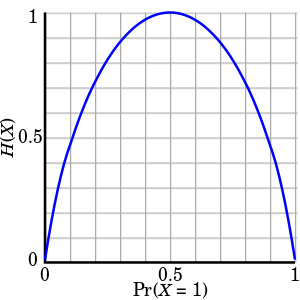
\includegraphics[scale=0.5]{img/entropy.png}
	\caption{Binary entropy function}
	\label{fig:entropy}
\end{figure}

The candidate functions, out of which the best on is chosen with the information gain, are \underline{randomly drawn}. Typically, one decides:
\begin{itemize}
    \item
        how many candidate functions are drawn
    \item
        if also linear projection of the data shall be drawn (e.g. consider only dimensions \(\{d_{i_1}, d_{i_2}, \dots, d_{i_n}\}\)
    \item
        how the splitting parameters are sampled
\end{itemize}
\(\Rightarrow\) Note that a sparser sampling leads to more "noise"/less optimal results. (\textit{Note:} might be desired, e.g. prevents overfitting)

Choice of tree depth:
\begin{itemize}
    \item
        set maximum depth ("mandatory")
    \item
        optional: set minimum number of samples for split 
    \item
        depending on the application, stop if for example 99\% of features in a node belong to one class
\end{itemize}

Final classifier output:
\begin{itemize}
    \item
        at a leaf node, report the relative frequencies of the class labels in that node (e.g., 15\%: class 1, 85\% class 2)
    \item
        combine al trees by averaging the individual tree outputs. If a single discrete label is required, decide for the class with maximum probability.
\end{itemize}

\section{Random Forests (continued)}
Example: Classification
\begin{enumerate}
    \item
        Randomly select a number of splitting functions 
    \item
        Evaluate the information gain for each splitting function
    \item
        Set the function with maximum information gain as the current nodes' decision function
    \item
        Recursively repeat for the child nodes, until max tree depth (or some other criterium) is reached 
\end{enumerate}

\subsection{Regression Forests}
Goal: predict a \underline{continous} label \(p(y|\vec{x})\). (Remark: choice of the model complexity is related to the bias/variance trade off)

"Leaf prediction model": a base function that is fitted to the samples. The leaf prediction model could be
\begin{multicols}{2}
\begin{itemize}
    \item
        constant
    \item
        linear
    \item
        polynomial
    \item
        ...
\end{itemize}
\end{multicols}

To faithfully represent all of the data with a single function, it would certainly make sense to use a polynomial model, or something even more complex. However, the random idea implies to subdivide/partition the space, and to fit simpler models to the individual partitions. As a specific example, let's split up our input data points:

\begin{figure}[ht]
	\centering
    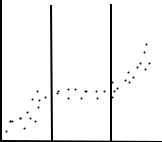
\includegraphics[height=4cm]{img/rf_regression.jpg}
	\caption{Regression split}
	\label{fig:rf_regression}
\end{figure}

The decision criterion for the splitting function works analogously to the classification case. The only difference ist that we need to define the entropy \(H(S_j)\) on continous values:
\[H(S_j) = -\frac{1}{\abs{S_j}} \cdot \sum_{\vec{x} \in S_j} \int_y p(y|x) \cdot log(y|x)dy\]
where \(p(y|x)\) can, e.g. be chosen as a Gaussian distribution \(p(y|x) = \mathcal{N}(y; \overline{y}(x), \sigma_y^2(x))\), where \(\overline{y}(x)\) is a linear function and \(\sigma_y(x)\) is the conditional variance computed from a linear fit.

%Probabilistic linear fit:
%\begin{figure}[H]
%	\centering
%    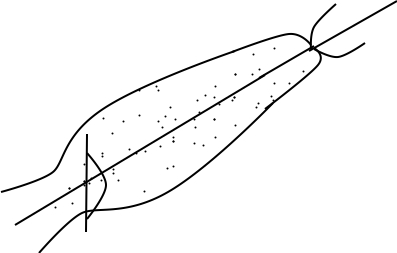
\includegraphics[height=4cm]{img/rf_linearfit.jpg}
%	\caption{Probabilistic linear fit}
%	\label{fig:rf_regression}
%\end{figure}

Combining the expression for \(p(y|x)\) into \(H(S_j)\) yields
\[H(S_j) = \frac{1}{\abs{S_j}} \cdot \sum_{\vec{x} \in S_j} \frac{1}{2} \cdot log((2 \pi e)^2 \sigma_y^2(\vec{x}))\]
\[\Rightarrow I(S_j, \vartheta) = \sum_{\vec{x} \in S_j} log(\sigma_y(\vec{x})) - \sum_{i \in \{L, R\}} (\sum_{x \in S_j^i} log (\sigma_y(\vec{x}))) \]

\subsection{Density Forests}
Very same idea, adapted to unlabelled data $\Rightarrow$ learning-baed density estimator.

Each leaf node is modeled as a multivariate Gaussian distribution. The information gain metric can again be reused, i.e. \(I(S_j, \vartheta) = H(S_j) - \sum_{i \in \{L, R\}} \frac{\abs{S_j^i}}{\abs{S_j}} \cdot H(S_j^i)\) but let us choose \(H(S_j)\) as
%Fancy
\[
H(S_j) = \frac{1}{2} \cdot log((2 \pi e)^d \abs{
    \underset{\mathllap{
        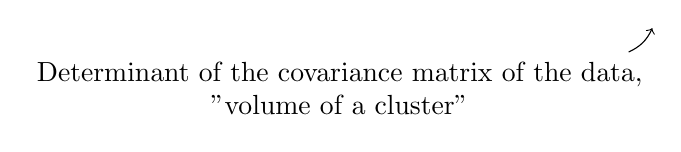
\begin{tikzpicture}
            \draw[->] (-0.3, 0) to[bend right=20] ++(0.3,2ex);
            \node[below left,align=center] at (0,0) {Determinant of the covariance matrix of the data,\\ "volume of a cluster"};
        \end{tikzpicture}
    }}{\Lambda} 
S_j})
\]

Plugging \(H(S_j)\) back into \(I(S_j, \vartheta)\) yields
\[I(S_j, \vartheta) = log (\abs{\Sigma(S_j)}) - \sum_{i \in \{L, R\}} \frac{\abs{S_j^i}}{\abs{S_j}} \cdot log(\abs{\Lambda(S_j^i)})\].

In each leaf, fit a multivariate Gaussian distribution to the data in that leaf using, e.g. MLE.

Note that the fitted densities have discontinuities at the splitting boundaries (this is the same type of discontinuity that we observed for regression forests or classification forests). However, remember that the result of a random forest is averaged over all individual trees. Because of randomization, each tree splits at a slightly different location, and thus the discontinuities are "averaged out" in the forest.


\section{Hidden Markov Models and Markov Random Fields}
Generative vs. Discriminative Model: let \(x\) denote the input, \(y\) the hidden variable/prediction/...
\[p(x,y) \Leftrightarrow p(y|x)\]

In a generative model, the available information is "more complete", i.e. we can for example also generate new samples \(x\) by sampling from \(p(x,y)\) by marginalizing over \(y\).

A discriminative model is slimmer (which is particularly useful for robust training with limited training data (the situation we're almost always in)); however, it only allows to discriminate between different \(y\)'s, but we can not generate new values \(x\).

\subsection{Remarks about HMMs}
\begin{itemize}
    \item
        Probabilistic, graphical model
    \item
        the directed edge in the graph can be understood as a statistical dependency: \[S_1 \rightarrow S_2 \Rightarrow p(S_2|S_1)\]
    \item
        Generative approach
    \item
        For many tasks, including speech processing, we oftentimes only allow for state transitions \(a_{ij}\) with \(i \leq j\). (no backward links) Those restricted HMMs are called "Left-right HMMs", as opposed to fully connected ("ergodic") HMMs.
\end{itemize}

\medbreak
How can we generate observations with an HMM?
\begin{enumerate}
    \item
        Sample from \(\pi = (\dots)\) (this gives you starting state) 
    \item
        Let \(S_1\) denote the starting state. Sample from \(b_1\) (column or row from production probability matrix \(B\)) a symbol
    \item
        Sample from \(\vec{a}_{S_1}\) (column or row from state transition matrix \(A\)) the next state
    \item
        Repeat 2.-3. until (randomly drawn/desired) word length reached
\end{enumerate}

\subsection{Markov Random Fields (MRF)}
1985, Geman/Geman: introduced MRFs to image processing:  Consider the pixel grid as a lattice (Gitter) of random variables.

More specifically, let us assume that the image \(F\) is given by the random matrix \([f_{ij}]\). %\(\Rightarrow p([f_{ij}])\). 

Assumption: limited statistical dependency:
\[p(f_{ij}| f_{i-1, j-1}, f_{i, j-1}, f_{i-1,j})\]
where \(f_{i-1, j-1}, f_{i, j-1}, f_{i-1,j})\) form a dependency of the neighbors to \(f_{i,j}\) (This will be our Markov property).

\[p([f_{ij}]) = \prod_{i,j} p(f_{i,j} | f_{i-1, j-1}, f_{i, j-1}, f_{i-1,j})\]

\subsubsection{Definition of MRF}
Lets us consider the features/observations \(\vec{x}_1,\vec{x}_2, \dots, \vec{x}_N\)
\begin{enumerate}
    \item
        Positivity: \(p(\vec{x}_1,\vec{x}_2, \dots, \vec{x}_N) > 0\)
    \item
        Markov property: \(p(\vec{x}_k | \vec{x}_1, \dots, \vec{x}_{k-1},\vec{x}_{k+1} \dots, \vec{x}_N) = p(\vec{x}_k|\mathcal{N}(\vec{x}_k))\) where \(\mathcal{N}(\vec{x}_k)\) denoted the neighborhood of \(\vec{x}_k\).
\end{enumerate}
Definition of the neighborhood: 
\begin{enumerate}
    \item
        \(\vec{x}_k \notin \mathcal{N}(\vec{x}_k)\)
    \item
        \(\vec{x}_i \in \mathcal{N}(\vec{x}_k) \Rightarrow \vec{x}_k \in \mathcal{N}(\vec{x}_i)\)
    \item
        \(\mathcal{N}(\vec{x}_k) = \{\vec{x}_i | 0 < dist(\vec{x}_i, \vec{x}_k) \leq t\}\)
\end{enumerate}
Example: Pixel grid:
\(\mathcal{N}(\vec{x}_{i,j}) = \{x_{k,l} | (i - k)^2 + (j - l)^2 \leq c^2, i \neq k \text{ or } j \neq l \}\)
\begin{itemize}
    \item
        NESW as neighbors, 4-Neighborhood \((c=1)\)
    \item
        All around as neighbors, 8-Neighborhood \((c=\sqrt 2)\)
\end{itemize}

\section{Markov Random Fields (continued)}
(Graph) clique: Complete subgraph

Gibbs Random Field (GRF): A GRF is given by the PDF 
\(p(x) = \frac{1}{
\underset{\mathllap{
        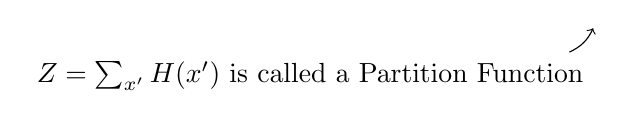
\begin{tikzpicture}
            \draw[->] (-0.3, 0) to[bend right=20] ++(0.3,2ex);
            \node[below left,align=center] at (0,0) {\(Z = \sum_{x'}H(x')\) is called a Partition Function};
        \end{tikzpicture}
    }}{Z}}  e^{-H(x)}\)
, where \(H(x)\) is an energy function, i.e. a sum of potential functions. For a given PDF \(p(x)\), the choice of energy function is not unique. Consider for example:
\[H(x) = - log p(x) - log Z \]
\[p(x) = \frac{1}{Z} e^{-H(x)} = \frac{1}{Z} e^{log p(x)} e^{log Z} = p(x)\]
\[\Rightarrow \text{we can chose Z arbitratily}\]

The interesting theoretical property is that GRF and MRF are equivalent. This is called the \textit{Hammersley-Clifford Theorem}.

\bigbreak

\subsection{Example: image denoising}
Given: Observed noisy image \([g_{ij}]\)

Hidden variables are the ideal (noiseless) images \([f_{ij}]\).

\textbf{Assumption 1:} the ideal image is spatially smooth \[p([f_{ij}]) = \frac{1}{Z} \cdot e^{-H([f_{ij}])}\] where \(H([f_{ij}]) = \sum_{ij} \norm{\Delta f_ij}_2^2\) (sum of squared gradients, computed over a neighborhood) (Note: Smoother image produces smaller \(H\), which maximizes \(p([f_{ij}])\).

\textbf{Assumption 2:} \([g_{ij}]\) is similar to \(f_{ij}\), but corrupted by additive Gaussian noise.
\[ p([g_{ij}]|[f_{ij}]) = \prod_{i,j} \frac{1}{\sqrt{2\pi} \sigma_{ij}} \cdot exp(-\frac{1}{2\sigma_{ij}^2} \cdot \underset{\text{energy function H}}{(f_{ij} - g_{ij})^2)}\]

With these two functions defined, we can solve for a MAP estimte for \(f\): 
\begin{align*}
    \underset{\text{estimated ideal image}}{[\hat{f}_{ij}]} &= \argmax_{[f_{ij}]} p([f_{ij}]|[g_{ij}])\\
    &= \argmax_{[f_{ij}]} p([g_{ij}]|[f_{ij}]) \cdot p([f_{ij}])\\
    &= \dots \text{(take log)}\\
    &= \argmin_{[f_{ij}]} \{\sum_{ij} \norm{\Delta f_{ij}}_2^2 + \sum_{ij} \lambda_{ij}(f_{ij} - g_{ij})^2\}
\end{align*}
\(\norm{\Delta f_{ij}}_2^2\): function of clique of size 2

Lecture slides: \url{https://www.slideshare.net/ykwang/markov-random-field-mrf} 

\section{Markov Random Fields}
\begin{figure}[ht]
	\centering
    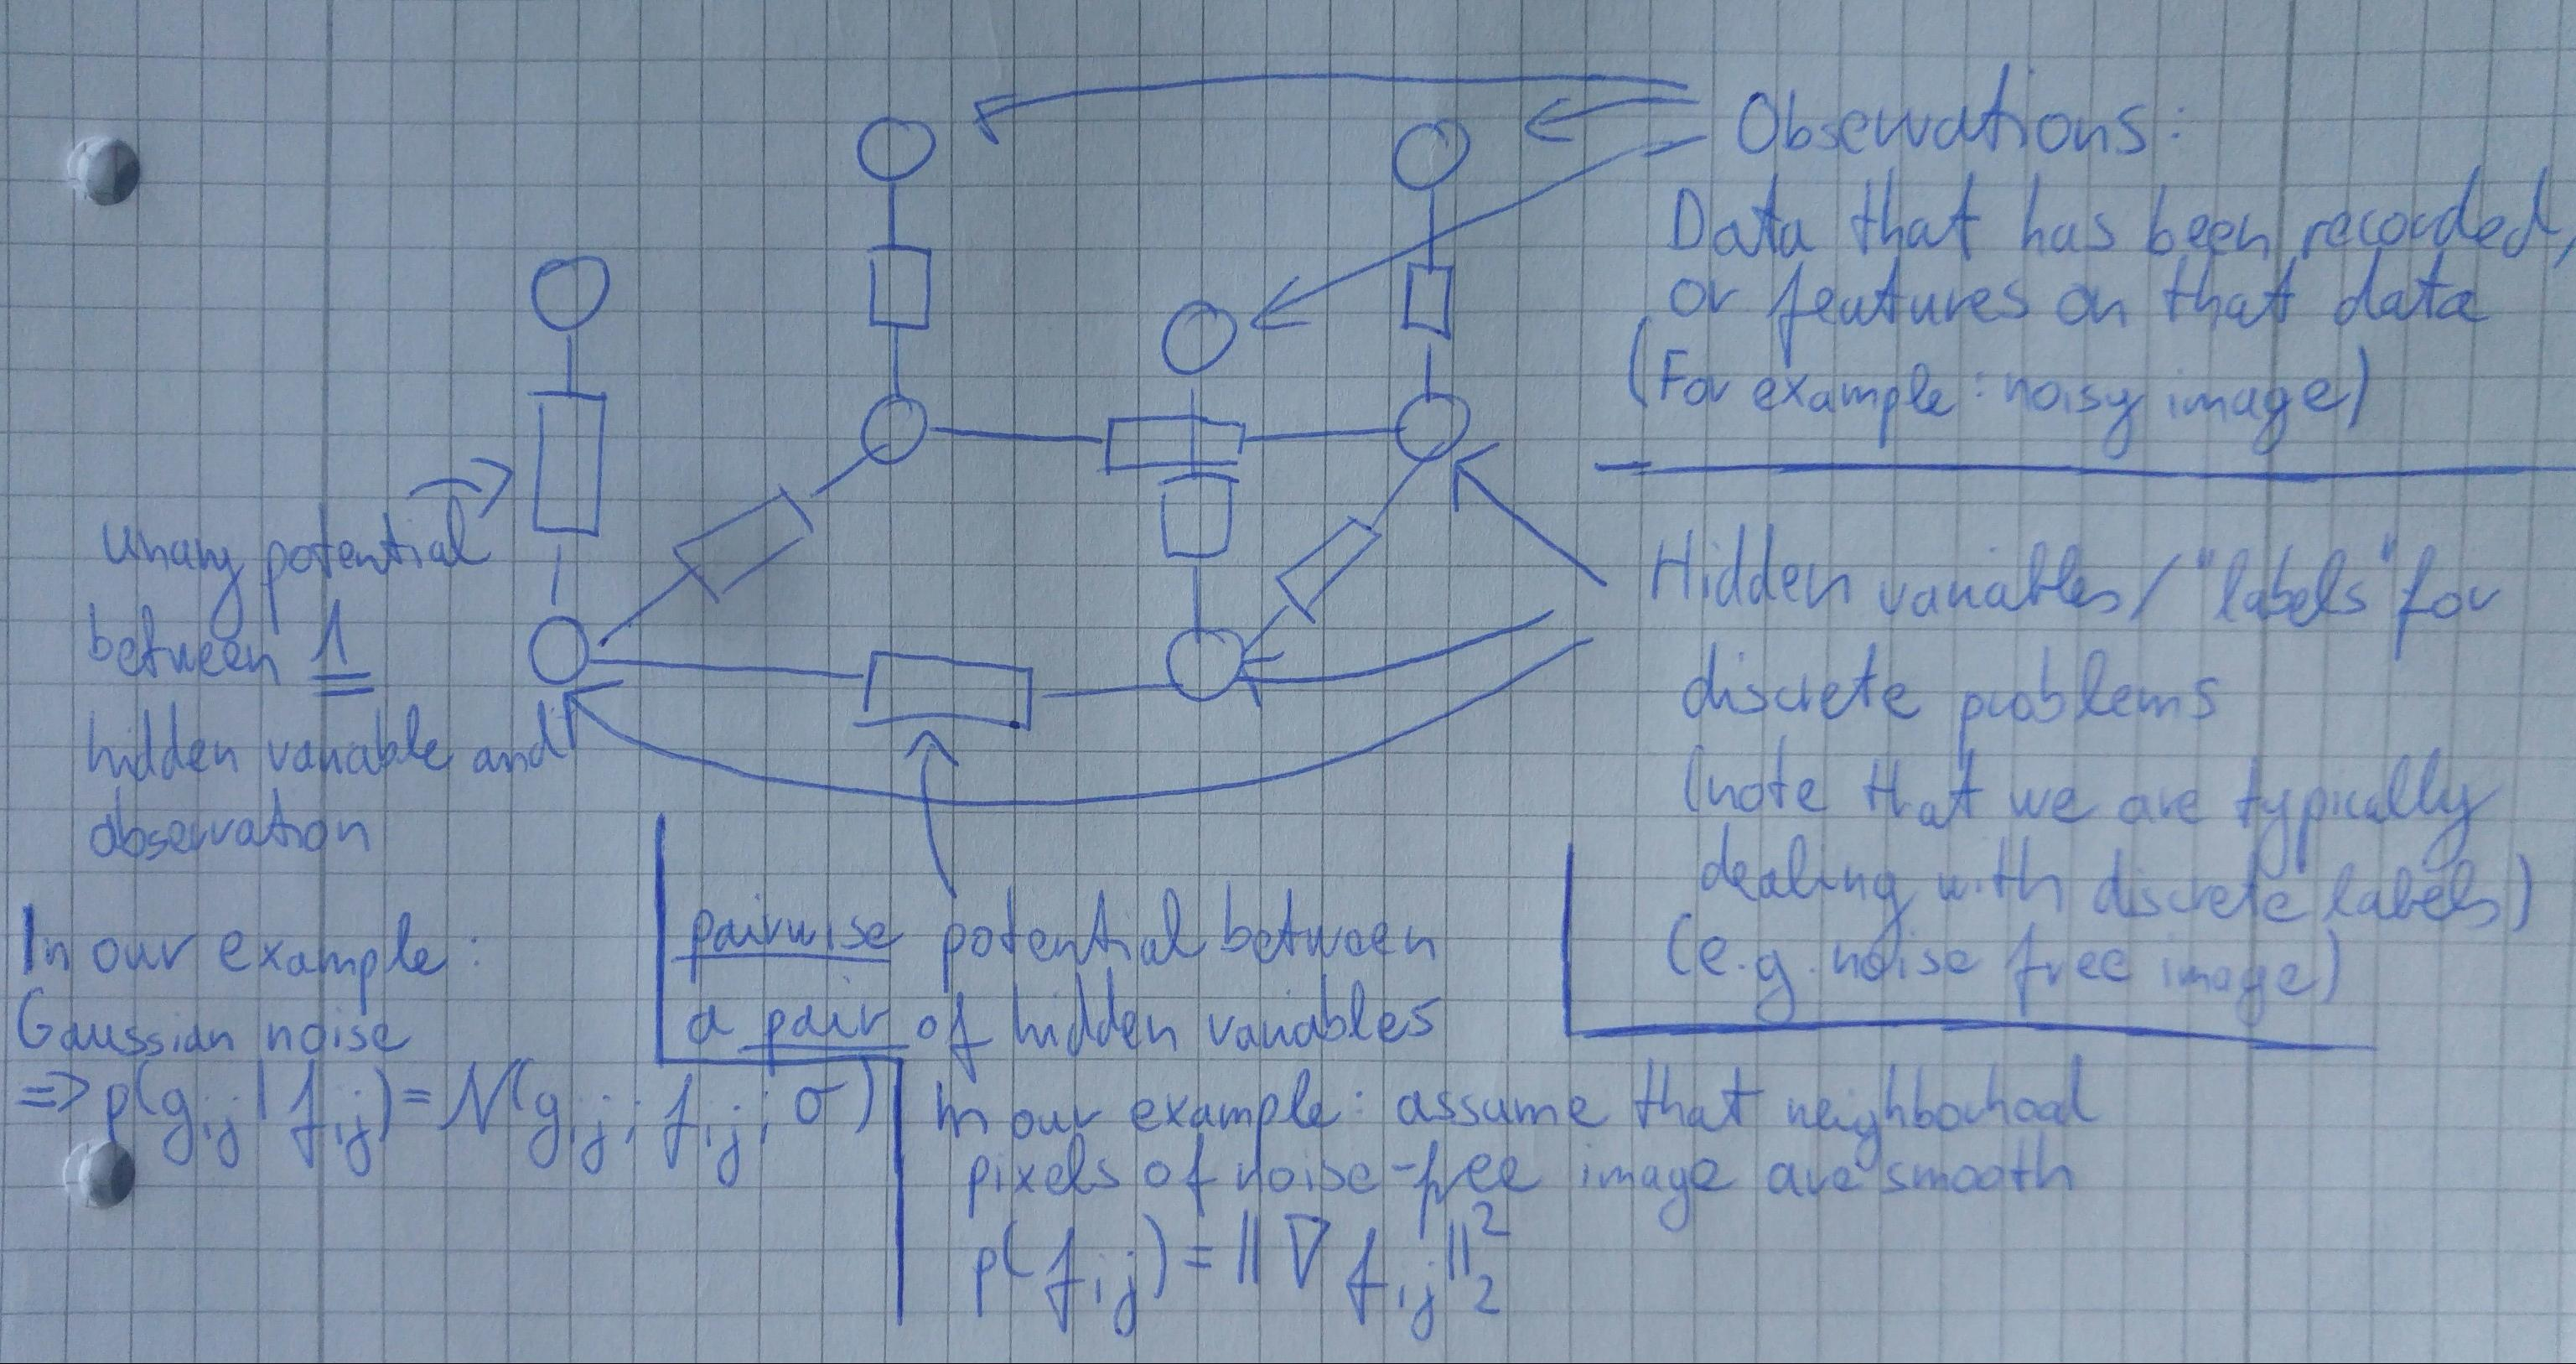
\includegraphics[scale=0.15]{img/mrf_1.jpg}
	\caption{MRF for image denoising}
	\label{fig:mrf_1}
\end{figure}

From a engineering perspective, we model the hidden variables by defining the unary and pairwise potentials. These are local relationships in the graph, i.e. they don't require complicated non-local interactions to be considered.

Remember from last week: a MRF and a GRF (Gibbs Random Field) are equivalent (\textit{Hammersley-Clifford} theorem).
This means that we can exchange the probabilities (defining the PDFs between the nodes in the MRF model might be impossible/hard) that describe the node relationships by potentials.

\[p(\vec{x}) = \prod_C p_C(\vec{x}_C) = \frac{1}{Z} \prod_C \psi_C(x_C)\]

Such potentials are much easier to design: We are typically interested in potential functions that assume a minimum value in a specific situation, e.g. \(\norm{\Delta f_{ij}}_2^2\) is minimal if \(f_{i,j} = f_{i,j+1} = \dots\), that depends on what we would like to achieve with the MRF.

\(p(x_1, \dots, x_N) = \prod \dots\) independent segments of the random variables \(x_1, \dots, x_N\)

General form of a Gibbs potential:
\begin{align*}
    p(\vec{x}) &= \frac{1}{Z} \prod_C \phi_C (\vec{x}_C)
    = \frac{1}{Z} \prod_C e^{-H(\vec{x}_C)}
    = \frac{1}{Z} e^{- \sum_C H(\vec{x}_C)}
\end{align*}
where \(H(\vec{x}_C) = \norm{\Delta f_{ij}}_2^2\) or \(H(\vec{x}_C) = \mathcal{N}(g_{ij}, f_{ij}, \sigma))\).

\bigskip

\(H(\vec{x}_C)\) is an energy function that is defined over clique potentials. Solvers for Markov Random Fields seek to directly minimize \(H(\vec{x}_C)\) instead of maximizing \(\psi_C(x_C)\).

A modern way of solving an MRF is via \underline{graph cuts}\footnote{ Kolmogorov, Zabih: "What Energy Functions Can Be Minimized via Graph Cuts?"}.

\subsection{Maximum Flow and Minimum Cut}
\begin{figure}[ht]
	\centering
    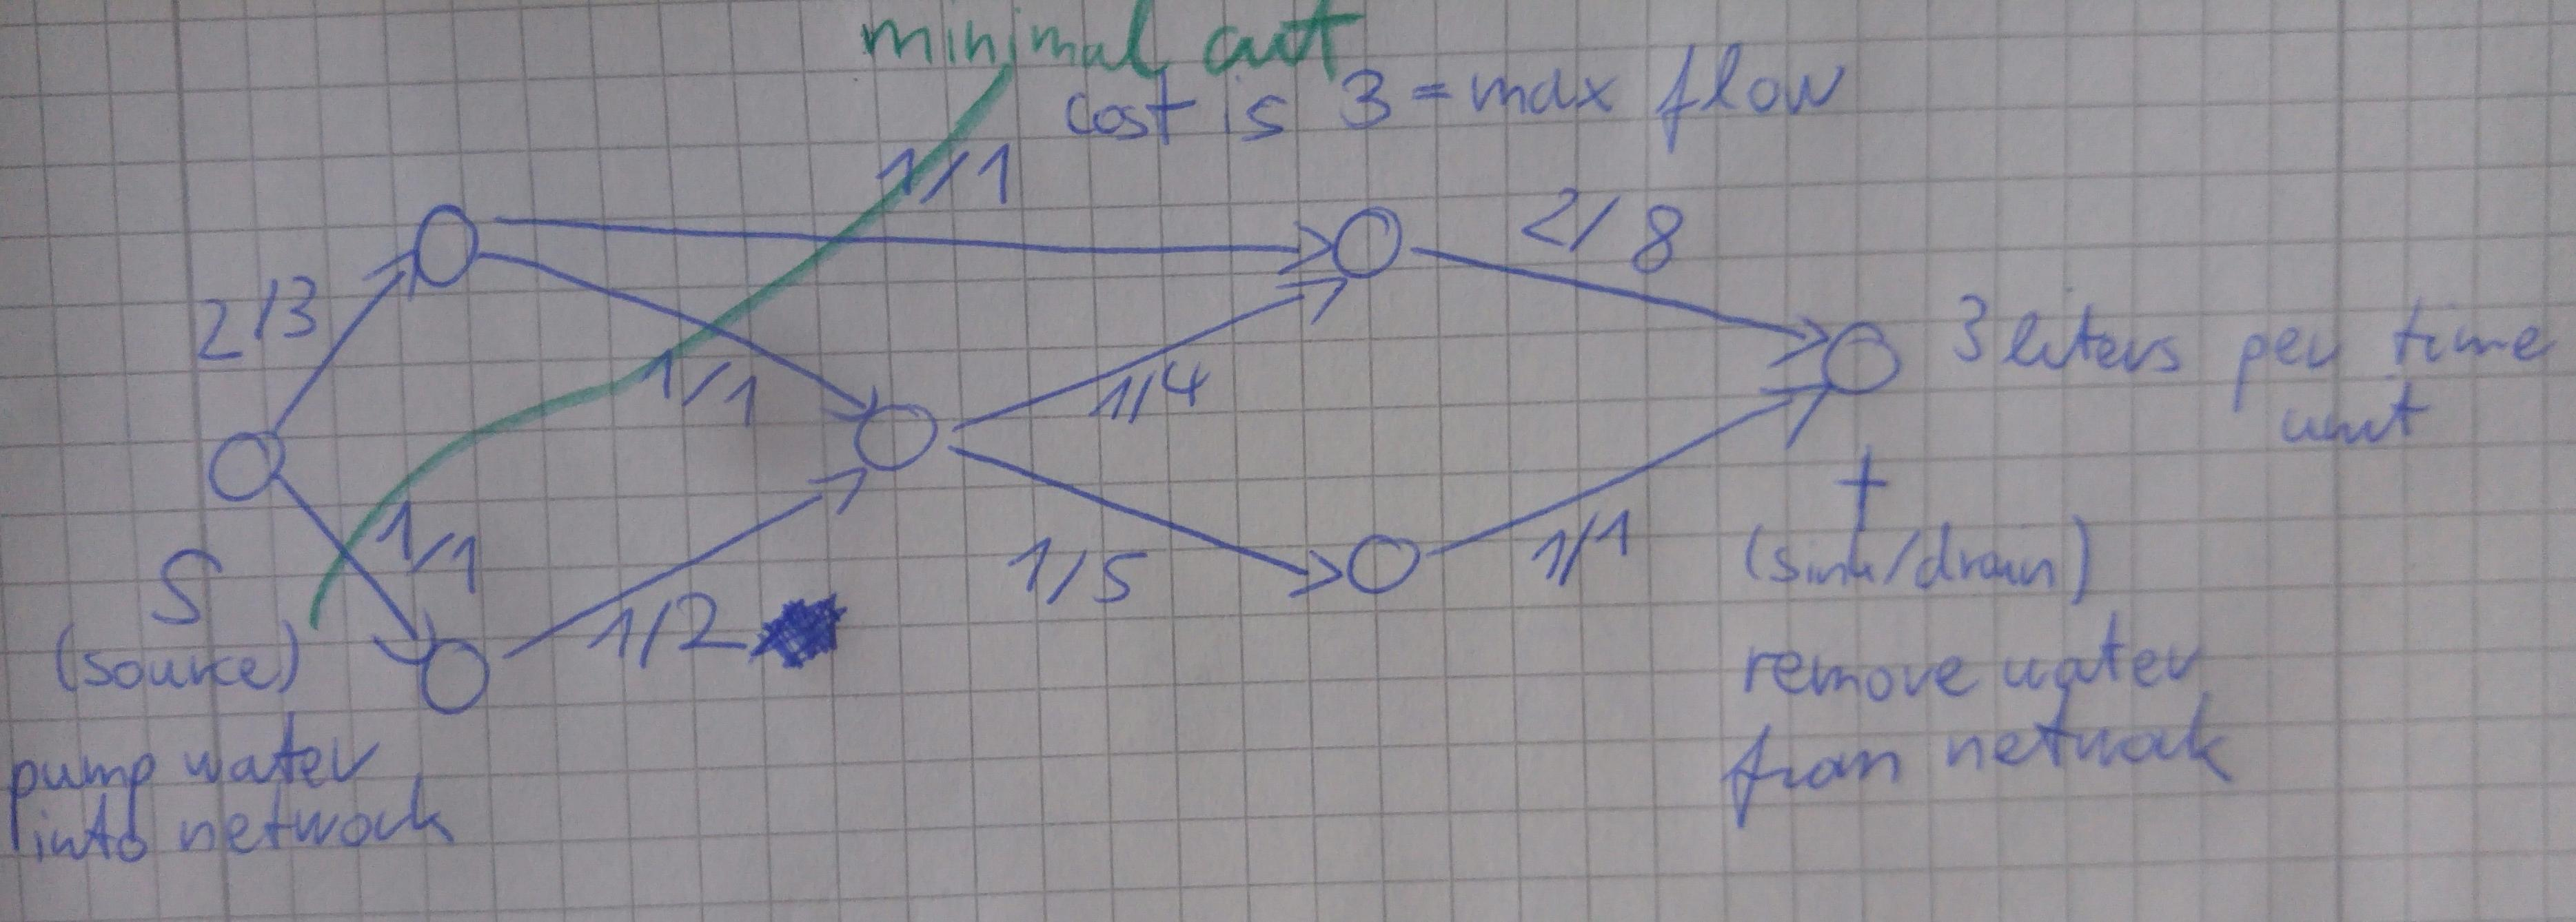
\includegraphics[scale=0.13]{img/mrf_2.jpg}
	\caption{Max Flow Min Cut}
	\label{fig:mrf_2}
\end{figure}

There are a number of classic algorithm that solve the max flow problem in polynomial time.

A minimum cut divides a network into two parts \(s, t\), such that the sum of the edge weights that are cut are minimal.

A solution to the maximum flow problem is a solution to the minimum cut problem: the minimum cut consists of edges that are fully used in the solution to the max flow problem.

\newpage
\begin{appendices}

\section{Lawrence R. Rabiner, Fellow: A Tutorial on Hidden Markov Models and Selected Applications in Speech Recognition}
\subsection{Discrete Markov Processes}
\begin{itemize}
    \item
        set of \(N\) discrete states \(S_1, S_2, \dots, S_N\)
    \item
        set of state transition probabilities \(a_{ij} = P(q_t = S_j | q_{t-1}=S_i)\)
%    \item
%        First order Markov chain: \(P(q_t = S_j|q_{t-1} = S_i, q_{t-2} = S_k, \dots) = P(q_t = S_j | q_{t-1}=S_i)\).
    \item
        properties: \(a_{ij} \geq = 0\) and \(\sum_{j=1}^N a_{ij} = 1\)
    \item
        the states itself are observable
    \item
        Calculating the probability of observations sequence given a model:
        \begin{align*}
            P(O|Model) &= P(S_3, S_3, S_1, S_1, S_3, S_2, S_3|Model)\\
            &= P(S_3) \cdot P(S_3|S_3) \dots P(S_3|S_2)\\
            &= \pi_3 \cdot a_{33} \dots a_{23}\\
            &= \dots
        \end{align*}
        where \(\pi_i = P(q_1 = S_i)\) is the initial state probability
\end{itemize}

\subsection{Extension to Hidden Markov Models}



\section[Undirected Graphical Models]{Undirected Graphical Models (Markov Random Fields) \protect\footnote{The Elements of Statistical Learning: Chapter 17, Undirected Graphical Models}}
\subsection{Introduction}
\begin{itemize}
    \item
        Consist of vertices (nodes) and edges joining some pairs of vertices
    \item
        Each vertex represents a random variable
    \item
        No edge between two vertices \(\Rightarrow\) conditionally independent, given the other variables
    \item
        Edges are parameterized by values or \textit{potentials} that encode the strength of the conditional dependence between the random variables
    \item
        Main challenges: model selection (structure), estimation of edge parameters from data (learning), and computation of marginal vertex probabilities and expectations, from their joint distribution (inference)
\end{itemize}

\subsection{Markov Graphs and Their Properties}
A graph \(\mathcal{G}\) consists of a pair \((V,E)\), where \(V\) is a set of vertices and \(E\) the set of edges (defined by pairs of vertices). Two vertices \(X\) and \(Y\) are called adjacent if there is a edge joining them; this is denoted by \(X \sim Y\). A \textit{complete graph} is a graph with every pair of vertices joined by an edge.

In a Markov graph \(\mathcal{G}\), the absence of an edge implies that the corresponding random variables are conditionally independent given the variables at the other vertices (known as \textit{pairwise Markov independencies} of \(\mathcal{G}\)). Notation:
\[\text{No edge joining } X \text{ and } Y \Leftrightarrow X \bot Y | \text{rest} \]
If \(A,B\) and \(C\) are subgraphs, then \(C\) is said to \textit{separate} \(A\) and \(B\) if every path between \(A\) and \(B\) intersects a node in \(C\). Separators have the nice property that they break the graph into conditionally independent pieces (known as \textit{global Markov properties} of \(\mathcal{G}\)). Notation:
\[\text{if } C \text{ separates } A \text{ and } B \text{ then } A \bot B |C\]

Pairwise and global Markov properties of a graph are equivalent. This is, the set of graphs with associated probability distributions that satisfy the pairwise Markov independencies and global Markov assumptions are the same. This is useful for inferring global independence relations from simple pairwise properties.

The global Markov property allows us to decompose graphs into smaller more manageable pieces and thus leads to essential simplifications in computation and interpretation. A \textit{clique} is a complete subgraph - a set of vertices that are all adjacent to one another (\textit{maximal} if no other vertices can be added to it).

A probability density function \(f\) over an Markov graph \(\mathcal{G}\) can be represented as
\[f(x) = \frac{1}{Z} \prod_{C \in \mathcal{C}} \psi_C(x_C)\]
where \(\mathcal{C}\) is the set of maximal cliques, and the postitive functions \(\psi_C(\cdot)\) are called \textit{clique potentials}. These are not in general density function, but rather are affinities that capture the dependence in \(X_c\) by scoring certain instances \(x_c\) higher than other. The quantity
\[Z = \sum_{x \in \mathcal{X}}\prod_{C \in \mathcal{C}} \psi_C (x_C)\]
is the normalizing constant, also known as \textit{partition} function.

This definition of \(f\) implies a graph with independence properties defined by the cliques in the product. This holds for Markov networks \(\mathcal{G}\) with positive distributions, and is known as the \textit{Hammersley-Clifford} theorem.

Because we are restricted to potential functions which are stritly positive it is convenient to express them as exponentials, so that
\[\psi_C(x_C) = exp(-E(x_C))\]
where \(E(x_C)\) is called an \textit{energy function}, and the exponential representation is called the \textit{Boltzmann distribution}. The joint distribution is defined as the product of potentials, and so the total energy is obtained by adding the energies of each of the maximal cliques.

\subsection{Image de-noising \protect\footnote{Bishop, Pattern Recognition: 8.3.3}}
Let the observed noisy image be described by an array of binary pixel values \(y_i \in \{-1, +1\}\), where the index \(i = 1, \dots, D\) runs over all pixels. We shall suppose that the image is obtained by taking  an unknown noise-free image, described by binary pixel values \(x_i \in \{-1, +1\}\) and randomly flipping the sign of pixels with some small probability.

Because the noise level is small, we know that there will be a strong correlation between \(x_i\) and \(y_i\). We also know that neighbouring pixels \(x_i\) and \(x_j\) in an image are strongly correlated.

\underline{TODO:} Random field model picture

This graph has two types of cliques, each of which contains two variables. The cliques \(\{x_i, y_i\}\) have an associated energy function that expresses the correlation between these variables (\(-\eta x_i y_i)\), where \(\eta\) is a positive constant) \(\Rightarrow\) lower energy (higher probability) when \(x_i\) and \(y_i\) have the same sign.

The remaining cliques comprise pairs of variables \(\{x_i, x_j\}\) where \(i, j\) are indices of neighbouring pixels. Again, we want the energy to be lower when the pixels have the same sign than when they have the opposite sign, and so we choose an energy given by \(-\beta x_i x_j\), where \(\beta\) is a positive constant.

Additionally, we add a term \(hx_i\) for each pixel \(i\) in the noise-free image. Such a term has the effect of biasing the model towards pixel values that have one particular sign in preference to the other.

The complete energy function for the model then takes the form
\[E(x,y) = h \sum_i x_i - \beta \sum{\{i,j\}} x_ix_j - \eta \sum_i x_i y_i\]
which defines a joint distribution over \(x\) and \(y\) given by
\[p(x,y) = \frac{1}{Z} exp\{-E(x,y)\}\]

\underline{\textit{Note:}}
\begin{align*}
    f(x) &= \frac{1}{Z} \prod_{C \in \mathbb{C}} \psi_C(x_C)\\
    &= \frac{1}{Z} \prod_{C \in \mathbb{C}} exp\{-E(x_C)\}\\
    &= \frac{1}{Z} exp\{-\sum_{C \in \mathbb{C}}E(x_C)\}
\end{align*}

We now fix the elements of \(y\) to the observed values given by the pixels of the noisy image, which implicitly defines a conditional distribution \(p(x|y)\) over noise-free images (see lecture).

\section{Density Estimation}
\subsection{Parzen windows:	Duda, Hart, Stork: "Pattern Classification", Section 4.3}
Common parametric density functions rarely fit the densities actually encountered in practice.

\textit{Nonparametric} procedures: can be used without the assumption that the forms of the underlying densities are known.

\subsubsection{Density estimation}
The proability \(P\) that a vector \(x\) will fall in a region \(\mathcal{R}\) is given by
\[P = \int_{\mathcal{R}} p(x') \ dx'.\]
where \(P\) is a smoothed or averaged version of the denisty function \(p(x)\).

Suppose that \(n\) samples \(x_1, \dots, x_n\) are drawn independently from \(p(x)\). We expect that the ratio \(k/n\), where \(k\) is the number of samples inside the region, will be a very good esimate for \(P\). This estimate is especially accurate when \(n\) is very large. If we now assume that \(p(x)\) is continous and that the region \(\mathcal{R}\) is so small that \(p\) does not vary consideratly within it, we can write
\[\int_{\mathcal{R}} p(x') dx' \simeq p(x) V,\]
where \(x\) is a point within \(\mathcal{R}\) and \(V\) is the volume enclosed by \(\mathcal{R}\). Combining all the equations:
\begin{align*}
    P &\simeq p(x) V\\
    k/n &\simeq p(x) V\\
    p(x) &\simeq \frac{k/n}{V}
\end{align*}

\subsubsection{Parzen Windows (Kernel density estimation)}
For now: \(R_n\) is a \(d\)-dimensional hypercube. If \(h_n\) is the length of an edge of that hypercube, then its volume is given by
\[V_n = h_n^d\]

In order to obtain an analytic expression for \(k_n\), we define the window function
\[\varphi(u) = 
\begin{cases} 
    1 & \abs{u_j} \leq 1/2, \ \ j = 1,\dots,d\\
    0 & otherwise
\end{cases}\]
where \(\varphi(u)\) indicates if \(u\) lies within a unit hypercube centered at the origin.

It follows that \(\varphi((x-x_i)/h_n)\) equals 1 if \(x_i\) falls within the hypercube of volume \(V_n\) centered at \(x\), and is zero otherwise.

The number of samples in this hypercube is therefore given by
\[k_n = \sum_{i=1}^{n} \varphi(\frac{x-x_i}{h_n})\]
and we obtain
\[p_n(x) = \frac{1}{n}\sum_{i=1}^{n}\frac{1}{V_n} \varphi(\frac{x-x_i}{h_n})\]

We don't have to restrict ourselfs to the hypercube window function (we can use for example Gaussian windows etc.). In essence, the window function is being used for \textbf{interpolation} - each samples contribution to the estimate in accordance with its disntace from \(x\).

We can rewrite this by defining a function 
\[\delta_n (x) = \frac{1}{V_n} \varphi (\frac{x}{h_n})\]
and then obtain \(p_n(x)\) as the average
\[p_n(x) = \frac{1}{n} \sum_{i=1}^N \delta_n(x-x_i)\]

\section{Comaniciu, Meer: "Mean Shift: A Robust Approach Toward Feature Space Analysis"}


\end{appendices}
\end{document}
